\section{Personnages}
Les personnages avec un ‘ \textbf{*} ’ sont des Jokers, ils possèdent un fiche de perso jouable. 

Par ordre d'apparition :

\begin{figure}[h!]
    \centering
    
\includegraphics[width=\linewidth]{_img/dos-au-muur/industrial-automaton.png}
    \caption{Industrial Automaton}
\end{figure}

\newpage
\subsection{Vyna Anen} \label{sec:vyna-anen}
\noindent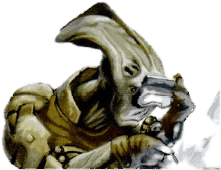
\includegraphics[width=\linewidth]{_img/dos-au-muur/vyna-anen.png}
\textbf{Race:} Sluissi

\subsubsection{Background}

Vyna Anen est l’un des agents de liaison entre Industrial Automaton et l’Empire. Officiellement employé par IA comme secrétaire au service des "Projets Spéciaux". 

Vyna est un homme pragmatique qui fait ce que l’Empire lui demande sans poser de questions, sans scrupules ni états d’âme. C’est un fin négociateur entièrement voué à l’Empire.

\subsubsection{Traits}

\begin{itemtable}[ c c c c c ]
    \textbf{Agi} & \textbf{Int} & \textbf{\^Ame} & \textbf{For} & \textbf{Vig} \\
    d6           & d10          & d6             & d4           & d6
\end{itemtable}
\begin{itemtable}[ l X ]
    \textbf{Allure}      & 6 \\
    \textbf{Compétences} & Intimidation d6, Persuasion d12, Réseaux d6
\end{itemtable}

\subsubsection{Défense}
\begin{itemtable}[ c c ]
    \textbf{Parade}     & \textbf{Résistance} \\
    2                   & 5 
\end{itemtable}

\clearpage
\subsection{R4-3D*} \label{sec:r4-3d}

\clearpage
\subsection{Tinon Dystra} \label{sec:tinon-dystra}
\begin{figure}[h!]
    \centering
    
\includegraphics[height=250pt]{_img/dos-au-muur/tinon-dystra.png}
    \caption{Tinon Dystra}
\end{figure}

\subsubsection{Background}
Ce personnage est mort quand débute le scénario mais il garde son importance car il est le lien entre les joueurs et l'alliance Rebelle.

Tinon est un membre de l'alliance rebelle envoyé en mission d'infiltration sur un vaisson de Industrial Automaton (Le \nameref{sec:pelican}) afin de découvrir ce qu'il s'y trame. Mais sa mission à mal tourné et il n'a plus donné aucune nouvelle. 

En fait il s'est infiltré à bord du Pelican alors que la maladie des \nameref{sec:rakghoul} était en train de s'y répandre. A bord du Pelican il s'est fait infecté et s'est transformé en Rakghoul lui-même. Son vaisseau, le \nameref{sec:nimbus} est resté à quai sur le Pelican.

Tinon avait une relation avec \nameref{sec:lindi-dangon}.

\newpage
\subsection{Lindi Dangon} \label{sec:lindi-dangon}
\begin{figure}[h!]
    \centering
    
\includegraphics[height=250pt]{_img/dos-au-muur/lindi-dangon.png}
    \caption{Lindi Dangon}
\end{figure}
\subsubsection{Background}
Lindi Dangon commande l'une des cellule de résistance dans la zone de Taris. C'est elle qui a ordonné la mission durant laquelle \nameref{sec:tinon-dystra} à disparut. Elle se sent d'autant plus coupable que Tinon était son amant et depuis sa disparition elle n'a de sesse de la retrouver. Elle garde espoir tant qu'elle n'a pas de preuve de sa mort.

\subsubsection{Traits}

\begin{itemtable}[ c c c c c ]
    \textbf{Agi} & \textbf{Int} & \textbf{\^Ame} & \textbf{For} & \textbf{Vig} \\
    d6           & d10          & d8             & d4           & d4           
\end{itemtable}
\begin{itemtable}[ l X ]
    \textbf{Allure}      & 6 \\
    \textbf{Compétences} & Intimidation d8, Persuasion d8, Réseaux d10, Tir d10, Combat d4 \\
    \textdb{Atouts}      & Commandement
\end{itemtable}

\subsubsection{Défense}
\begin{itemtable}[ c c ]
    \textbf{Parade}     & \textbf{Résistance} \\
    5                   & 3 
\end{itemtable}

\newpage
\subsection{Garan Keggle}  \label{sec:garan-keggle}

\newpage
\subsection{Gil Harend}  \label{sec:gil-harend}

Persuasion : 5

\newpage
\subsection{Pulsipher} \label{sec:pulsipher}